\section{Frontend Architecture}

The frontend architecture focuses on responsive design, smooth navigation, and visually attractive layouts. Although the application uses traditional server-side rendering through Django templates, the interface is designed to simulate modern single-page application behavior through JavaScript-driven interactions.

Frontend technologies include:

\begin{itemize}
    \item \textbf{HTML5}: Semantic markup and form structure
    \item \textbf{CSS3}: Custom styling, responsive grid layouts, and animations
    \item \textbf{JavaScript}: Asynchronous form submission via Fetch API and dynamic DOM manipulation
    \item \textbf{Django Template Language}: Server-side data binding and template inheritance
\end{itemize}

\begin{figure}[H]
    \centering
    \begin{adjustbox}{max width=\textwidth}
    \begin{tikzpicture}[
        node distance=1.2cm and 0.8cm,
        box/.style={draw, rectangle, fill=purple!5, text width=2.2cm, align=center, rounded corners, minimum height=0.8cm, font=\small},
        arrow/.style={-latex, thick}
    ]
        \node (resp) [box] {Receive JSON};
        \node (parse) [box, right=of resp] {Parse Data};
        \node (dom) [box, right=of parse] {Update DOM};
        \node (img) [box, right=of dom] {Dynamic Images};
        \node (render) [box, right=of img] {Render UI};
        
        \draw [arrow] (resp) -- (parse);
        \draw [arrow] (parse) -- (dom);
        \draw [arrow] (dom) -- (img);
        \draw [arrow] (img) -- (render);
    \end{tikzpicture}
    \end{adjustbox}
    \caption{Frontend Rendering Workflow}
    \label{fig:frontend-workflow}
\end{figure}

\subsection{Responsive Design Features}

The application supports a wide range of devices:

\begin{itemize}
    \item \textbf{Desktop}: Full-width layouts with multi-column grids
    \item \textbf{Tablets}: Adaptive column collapsing with fluid widths
    \item \textbf{Smartphones}: Single-column stacked layouts with touch-friendly navigation
\end{itemize}

Responsive layouts are achieved through:

\begin{itemize}
    \item Flexible grid systems using CSS Flexbox and Grid
    \item Adaptive image scaling with \texttt{max-width: 100\%}
    \item Media queries for breakpoint-specific styling
    \item Mobile-friendly navigation with hamburger menu support
\end{itemize}

\subsection{Dynamic Destination Images}

To improve visual appeal, the application integrates fallback destination images using the \textbf{Unsplash Source API}. If local images are unavailable, the system dynamically loads travel-related images based on destination names. This feature enhances visual engagement, user immersion, and destination attractiveness.

\section{Key Application Interfaces}

\subsection{Landing and Authentication Pages}

The landing page acts as the entry point of the application and focuses on user engagement, travel inspiration, easy navigation, and quick registration access. The page features a hero section with a full-width background, a destination carousel showcasing popular Indian travel locations, and an inline trip planning form.

\begin{figure}[H]
    \centering
    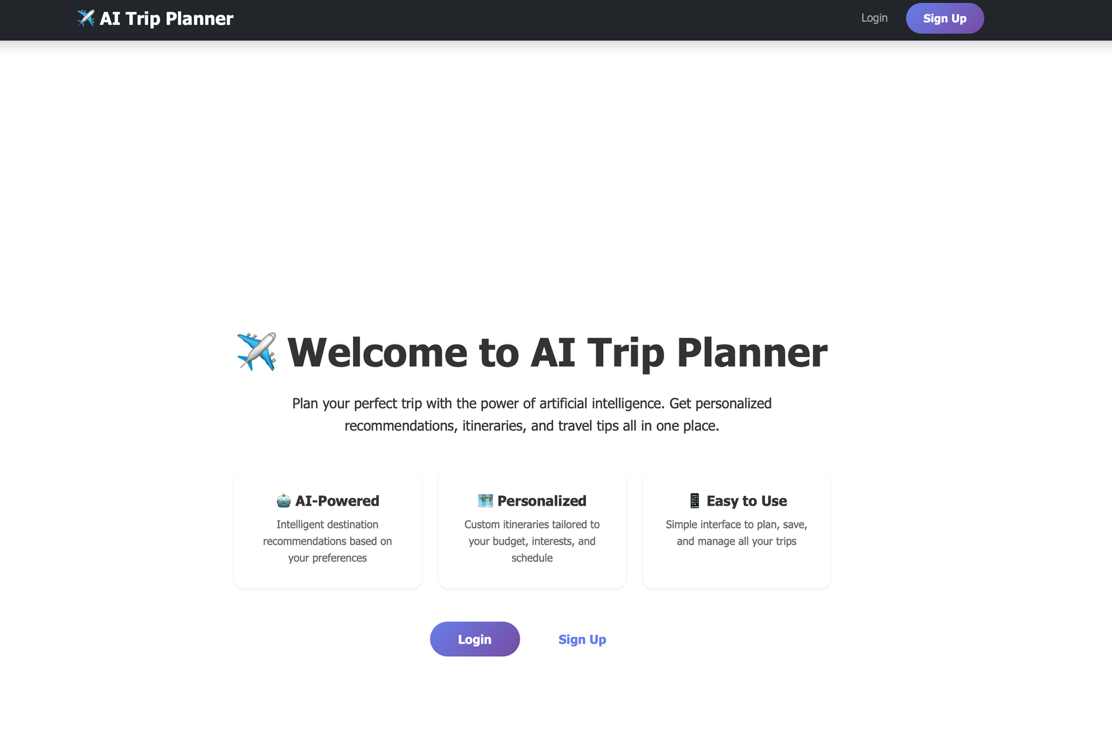
\includegraphics[width=0.9\textwidth,height=0.7\textheight,keepaspectratio]{images/Home page.png}
    \caption{Home Page Interface}
    \label{fig:screenshot-home}
\end{figure}

\begin{figure}[H]
    \centering
    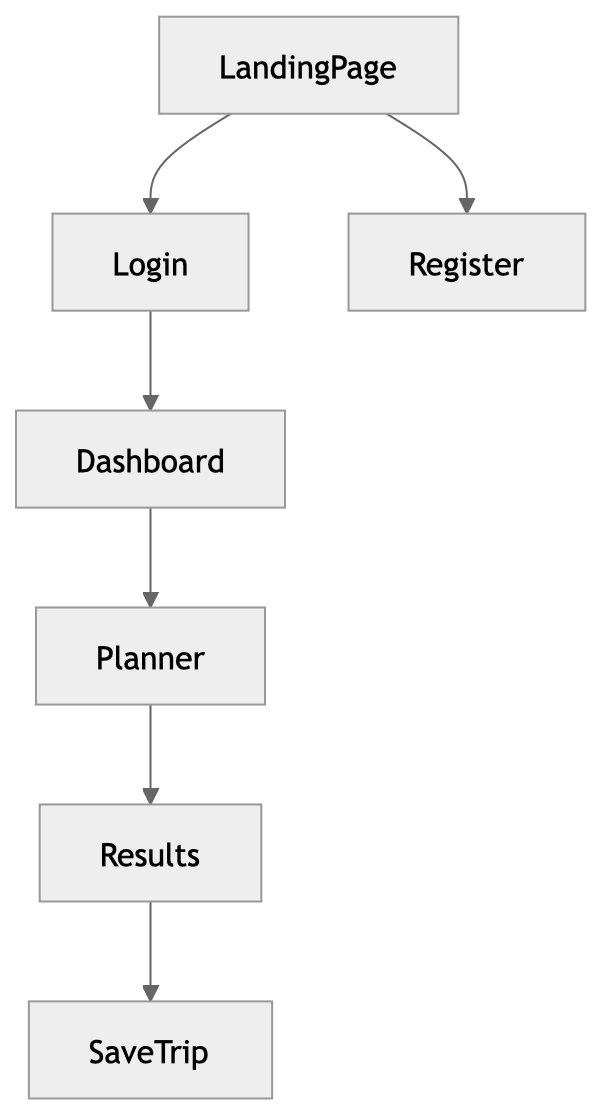
\includegraphics[width=0.9\textwidth,height=0.7\textheight,keepaspectratio]{images/User Navigation Structure.png}
    \caption{User Navigation Structure}
    \label{fig:nav-structure}
\end{figure}

Authentication pages include:
\begin{itemize}
    \item \textbf{Login form}: Username and password fields with CSRF protection
    \item \textbf{Registration form}: Username, email, and password with confirmation
    \item \textbf{Password validation}: Minimum length and confirmation matching
    \item \textbf{Session management}: Persistent login sessions with secure cookies
\end{itemize}

\begin{figure}[H]
    \centering
    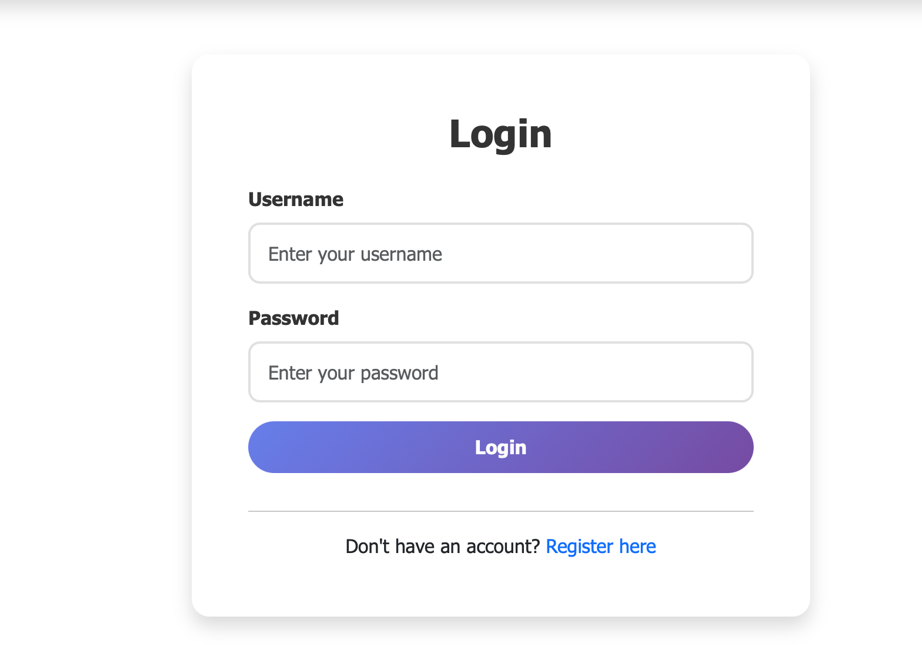
\includegraphics[width=0.85\textwidth,height=0.7\textheight,keepaspectratio]{images/Login page.png}
    \caption{Login Interface}
    \label{fig:screenshot-login}
\end{figure}

\begin{figure}[H]
    \centering
    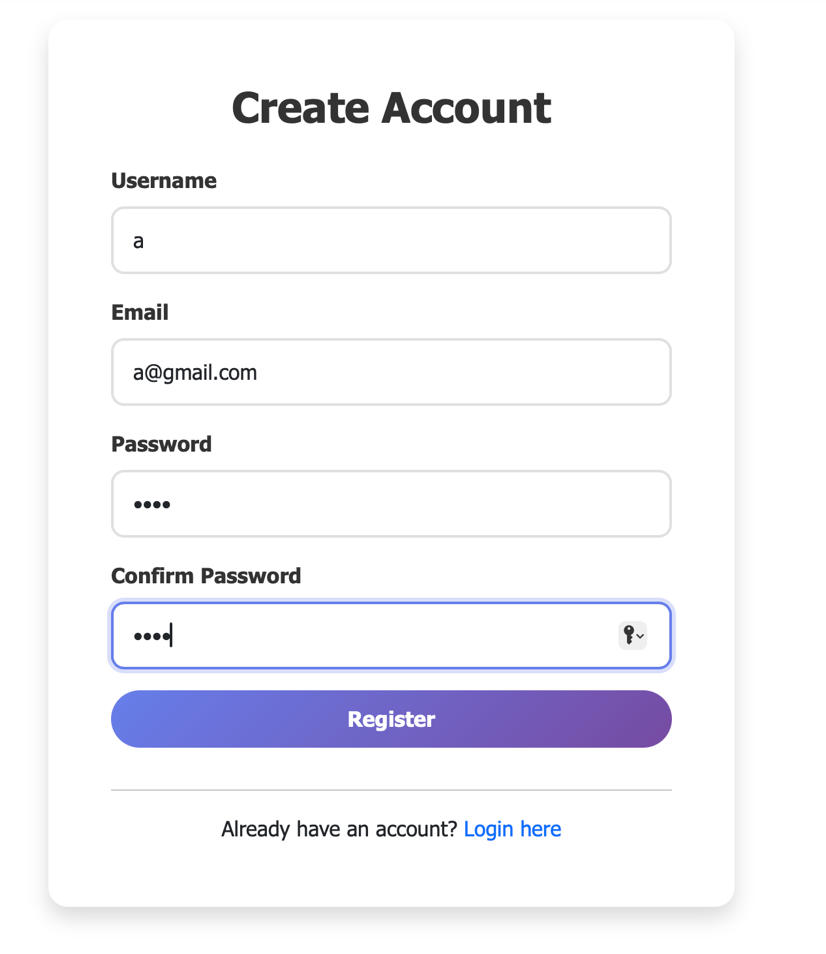
\includegraphics[width=0.85\textwidth,height=0.7\textheight,keepaspectratio]{images/Registration page.png}
    \caption{Registration Interface}
    \label{fig:screenshot-registration}
\end{figure}

\subsection{Destinations Explorer}

The destination explorer displays all 36 travel destinations using responsive card-based grid layouts. Each destination card contains:

\begin{itemize}
    \item Destination image (local or dynamically loaded from Unsplash)
    \item Climate information badge
    \item Estimated budget range
    \item Travel category tag
    \item Short destination description
    \item Quick link to the trip planning form pre-filled with the destination
\end{itemize}

The explorer supports real-time client-side filtering by destination name search and climate type selection, enabling users to find relevant destinations efficiently.

\begin{figure}[H]
    \centering
    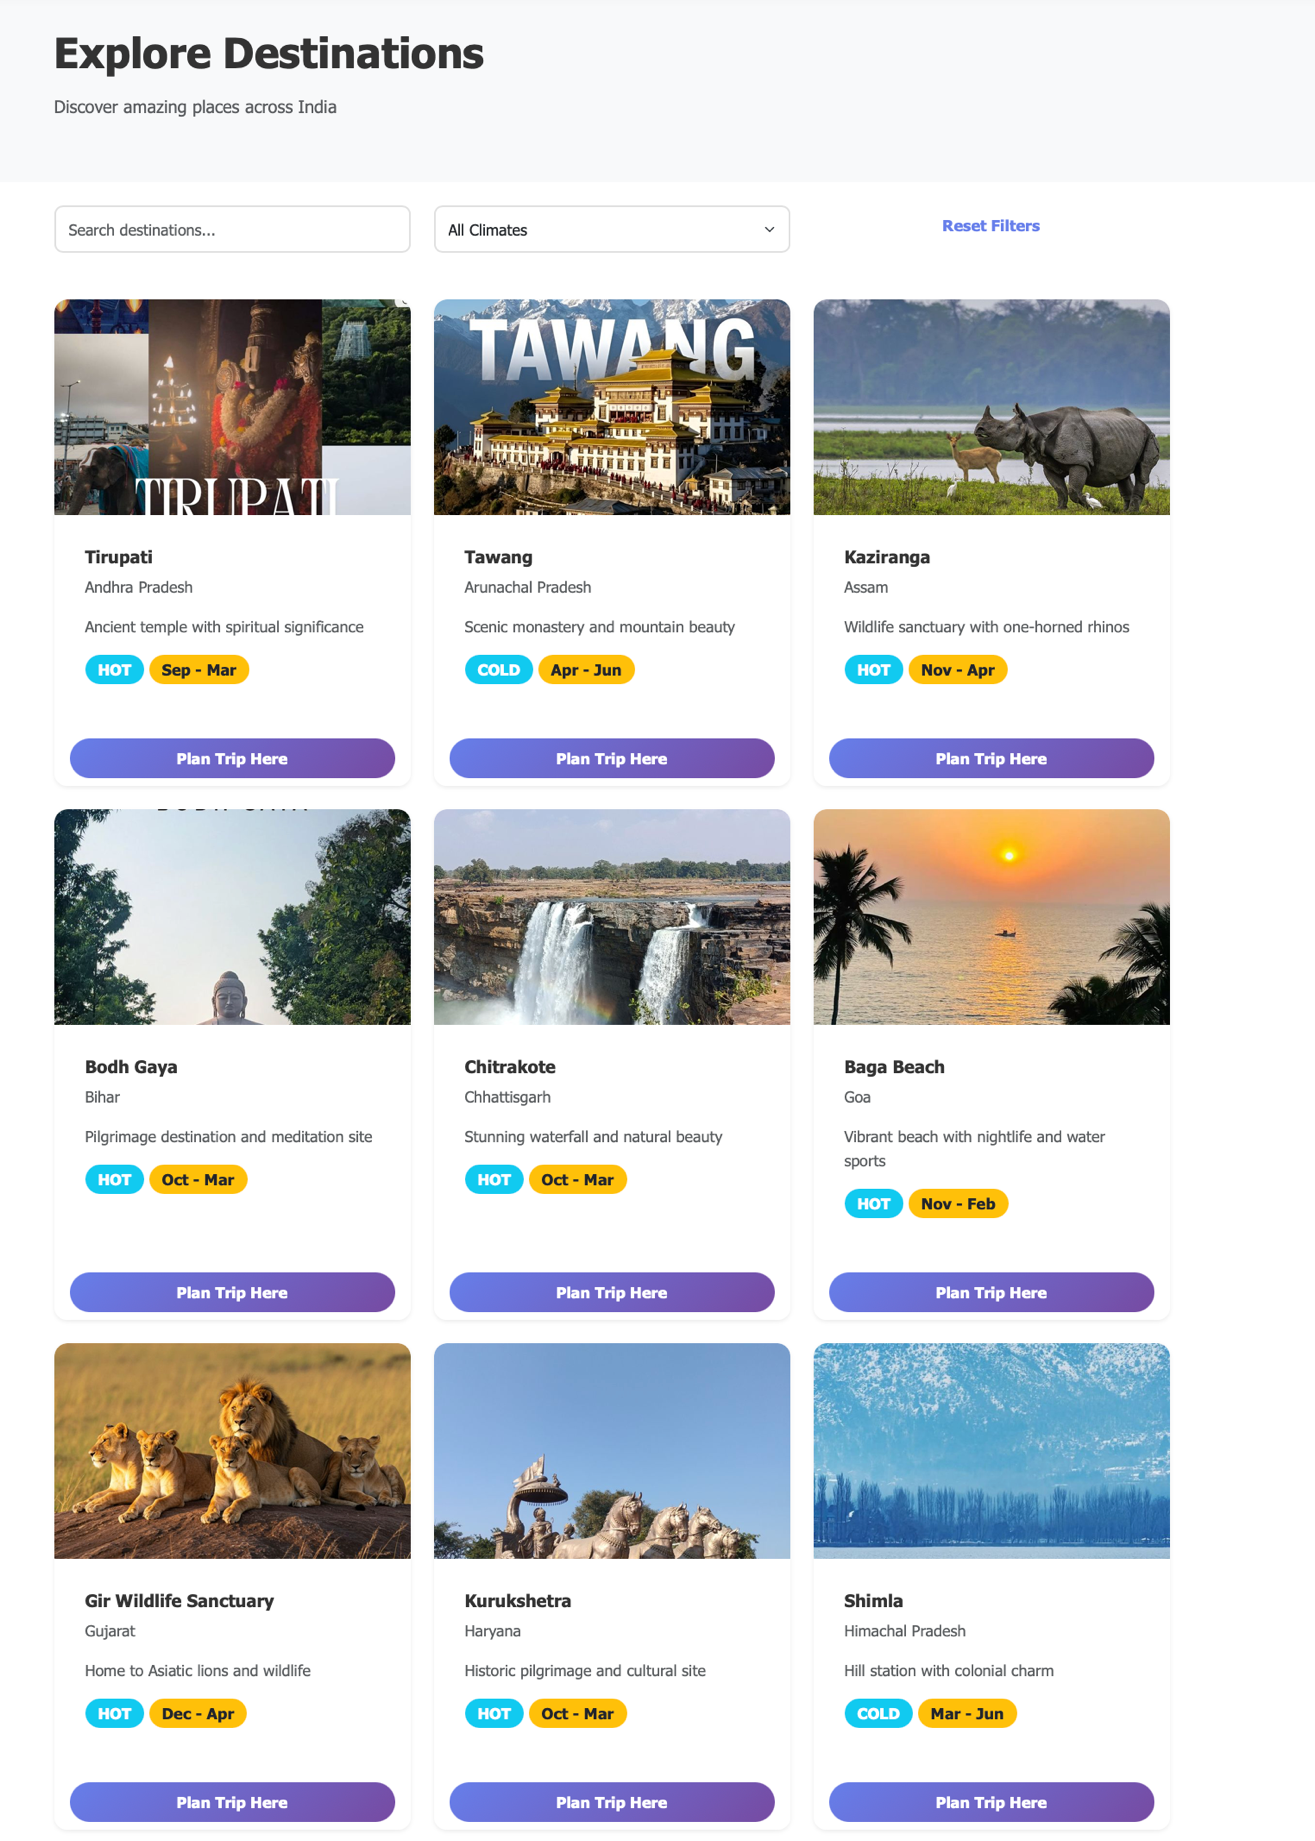
\includegraphics[width=0.9\textwidth,height=0.7\textheight,keepaspectratio]{images/Destinatioj explorer.png}
    \caption{Destinations Explorer Interface}
    \label{fig:screenshot-explorer}
\end{figure}

\subsection{Trip Planning Form}

The trip planning form acts as the primary interaction point for recommendation generation. The form securely collects:

\begin{itemize}
    \item \textbf{Budget}: Numeric input in INR with minimum value validation
    \item \textbf{Travel Days}: Integer selector (1--30 days)
    \item \textbf{Climate Preference}: Dropdown selection (Hot, Cold, Moderate)
    \item \textbf{Travel Type}: Dropdown selection (Adventure, Relaxation, Cultural, Family)
\end{itemize}

Interactive dropdowns and client-side validation improve user input accuracy and usability. Form submission is handled asynchronously via the JavaScript Fetch API, providing a seamless user experience without full page reloads.

\begin{figure}[H]
    \centering
    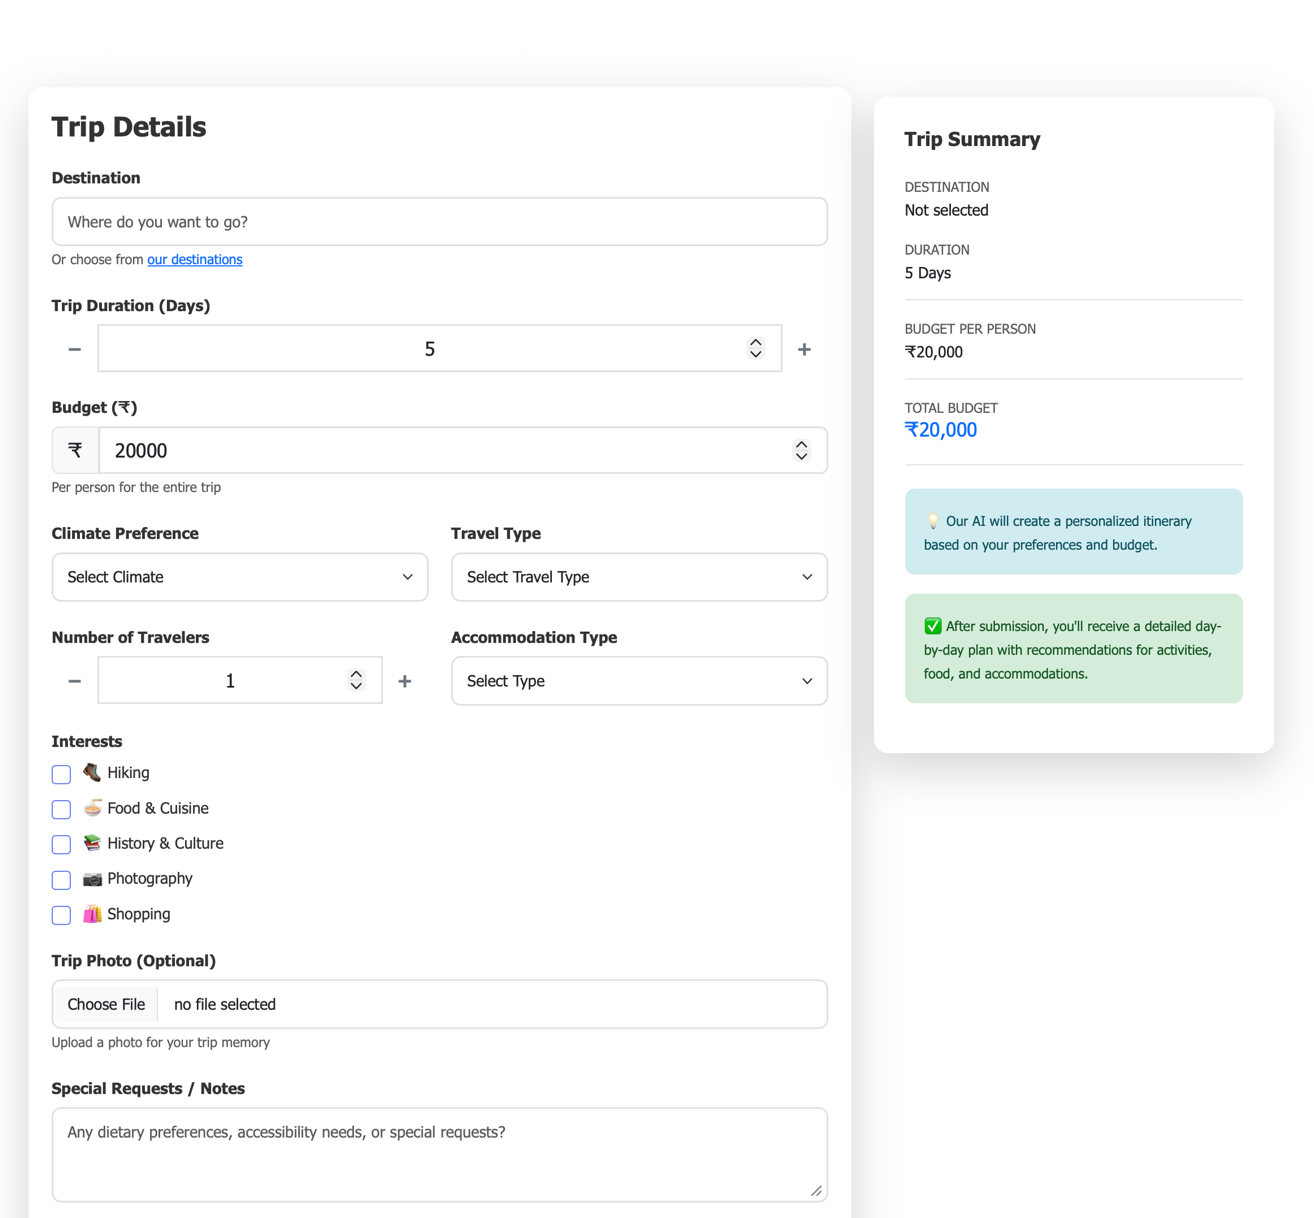
\includegraphics[width=0.9\textwidth,height=0.7\textheight,keepaspectratio]{images/Trip Planning Form.png}
    \caption{Trip Planning Form Interface}
    \label{fig:screenshot-form}
\end{figure}

\subsection{Dashboard (My Trips)}

The dashboard provides personalized trip management features including:

\begin{itemize}
    \item \textbf{Saved Itineraries}: Tabular display of all saved trip plans with destination images
    \item \textbf{Travel History}: Date-stamped records with budget and travel type information
    \item \textbf{Soft-Delete Functionality}: Trips moved to a ``Recently Deleted'' section rather than permanently erased
    \item \textbf{Trip Restoration}: Deleted trips can be recycled back to the active list
\end{itemize}

\begin{figure}[H]
    \centering
    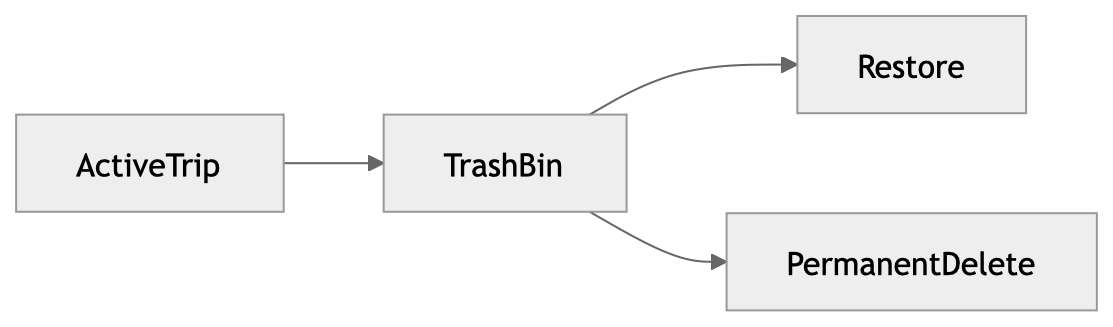
\includegraphics[width=0.9\textwidth,height=0.7\textheight,keepaspectratio]{images/Soft Delete Workflow.png}
    \caption{Soft Delete Workflow}
    \label{fig:soft-delete}
\end{figure}

The soft-delete mechanism prevents accidental data loss by setting the \texttt{is\_deleted} flag to \texttt{True} and recording the deletion timestamp in \texttt{deleted\_at}. The active trips query filters for records where \texttt{is\_deleted=False}.

\subsection{Results View}

The results interface displays the complete trip plan generated by the AI recommendation engine:

\begin{itemize}
    \item \textbf{Predicted Destination}: Name and destination image
    \item \textbf{Budget Summaries}: Total budget with percentage distribution across categories
    \item \textbf{Daily Itinerary Schedules}: Day-by-day activity plan
    \item \textbf{Activity Suggestions}: Recommended attractions and experiences
    \item \textbf{Travel Guidance}: Practical tips for the recommended destination
\end{itemize}

\begin{figure}[H]
    \centering
    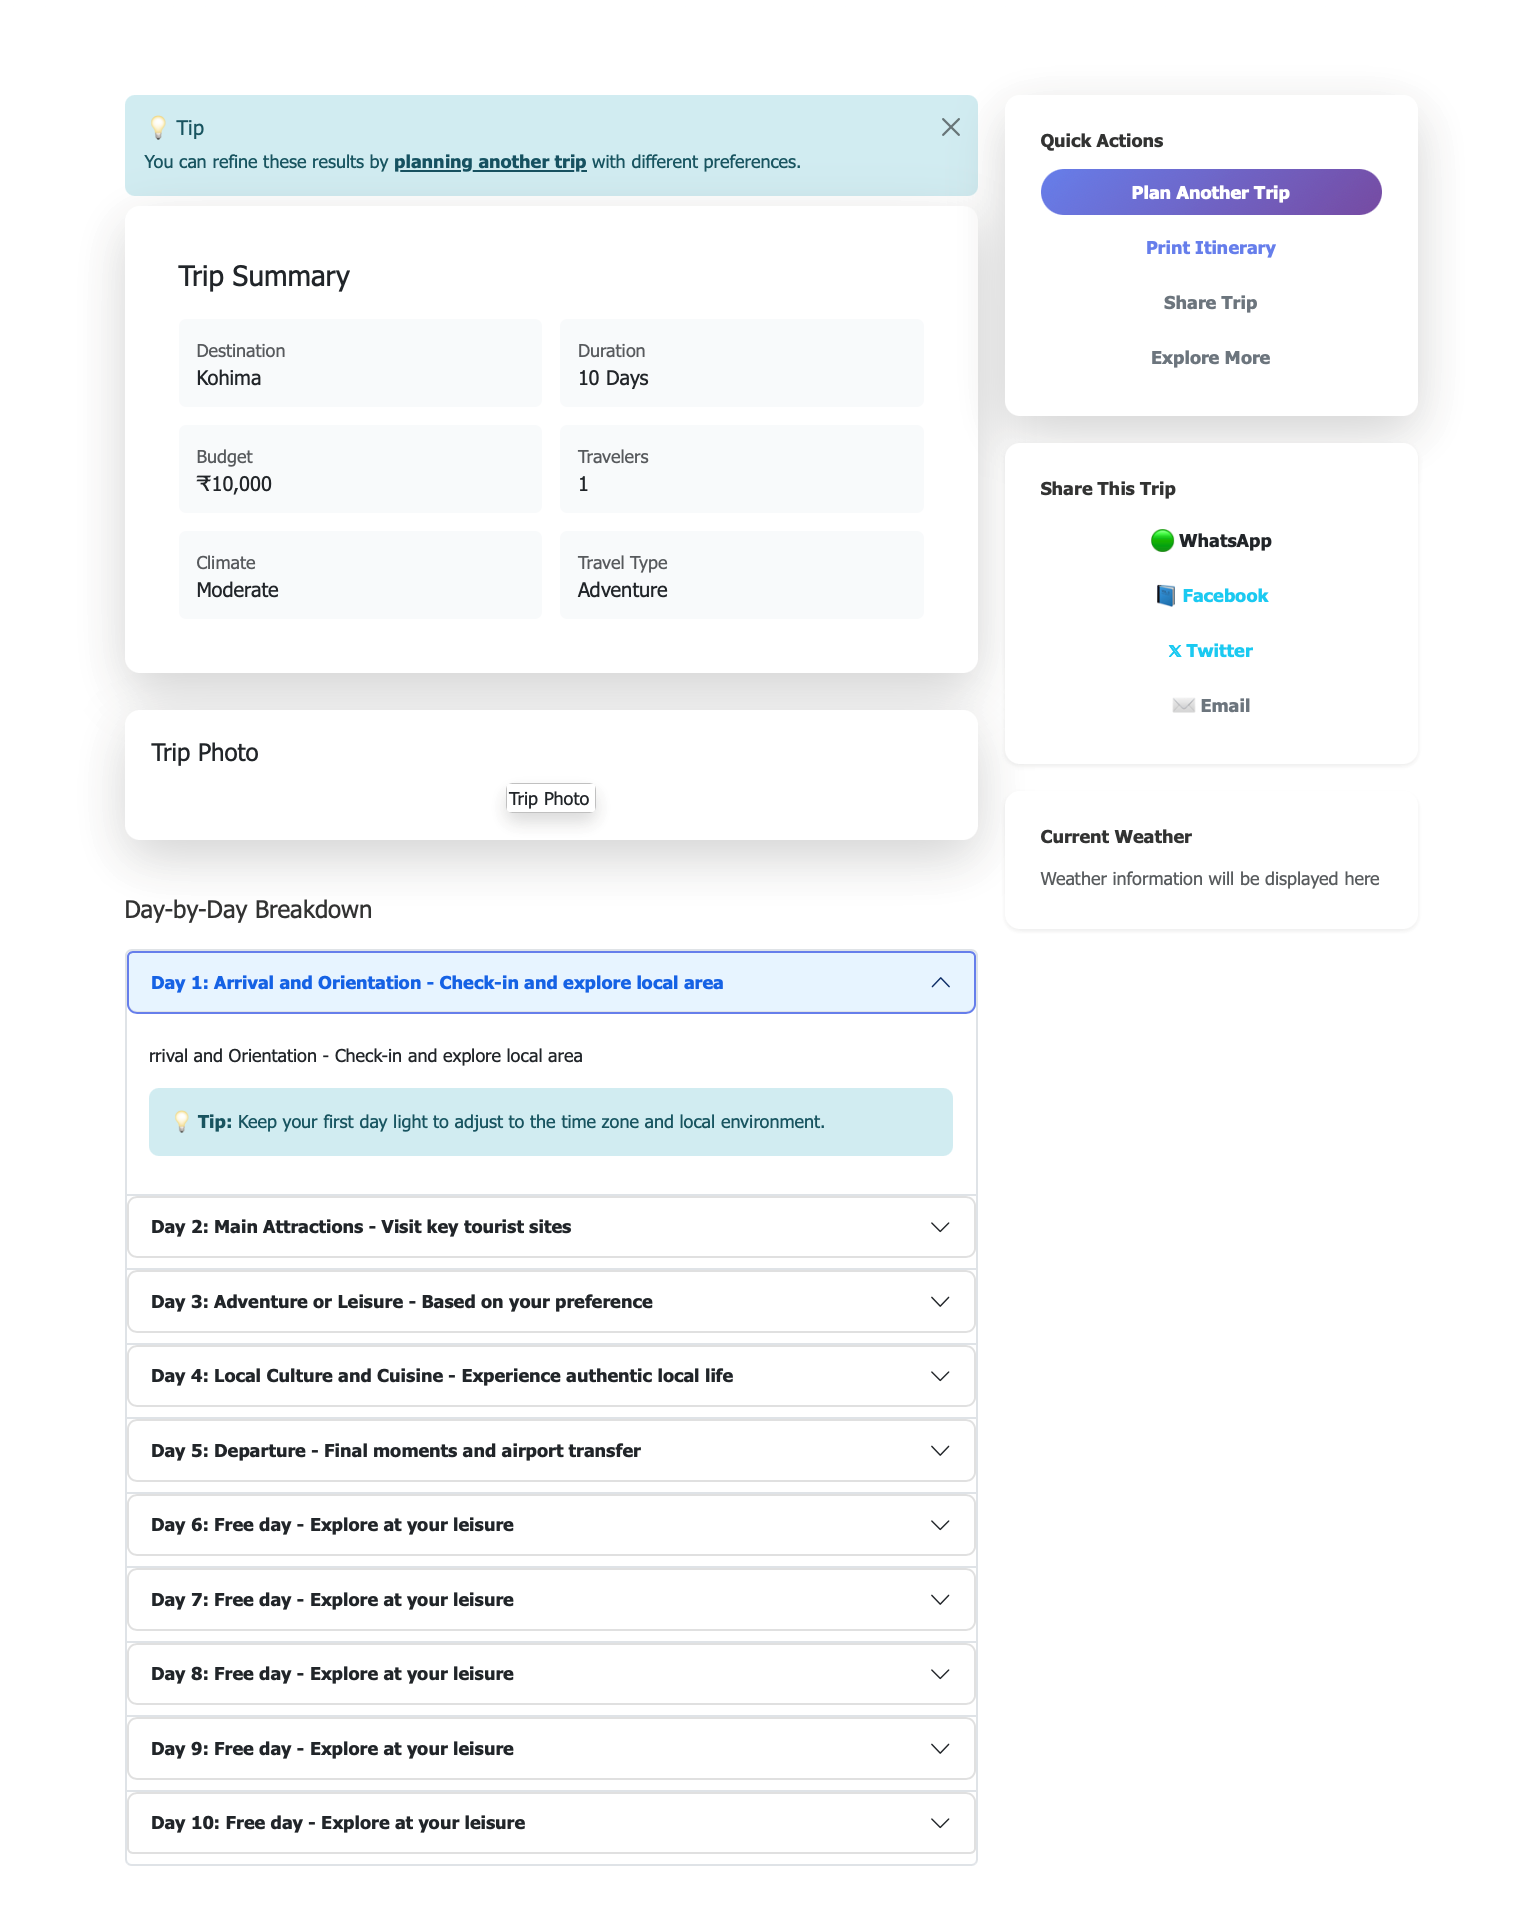
\includegraphics[width=0.9\textwidth,height=0.7\textheight,keepaspectratio]{images/Result View 1.png}
    \caption{Results View - Destination Recommendation and Cost Breakdown}
    \label{fig:screenshot-result-1}
\end{figure}

\begin{figure}[H]
    \centering
    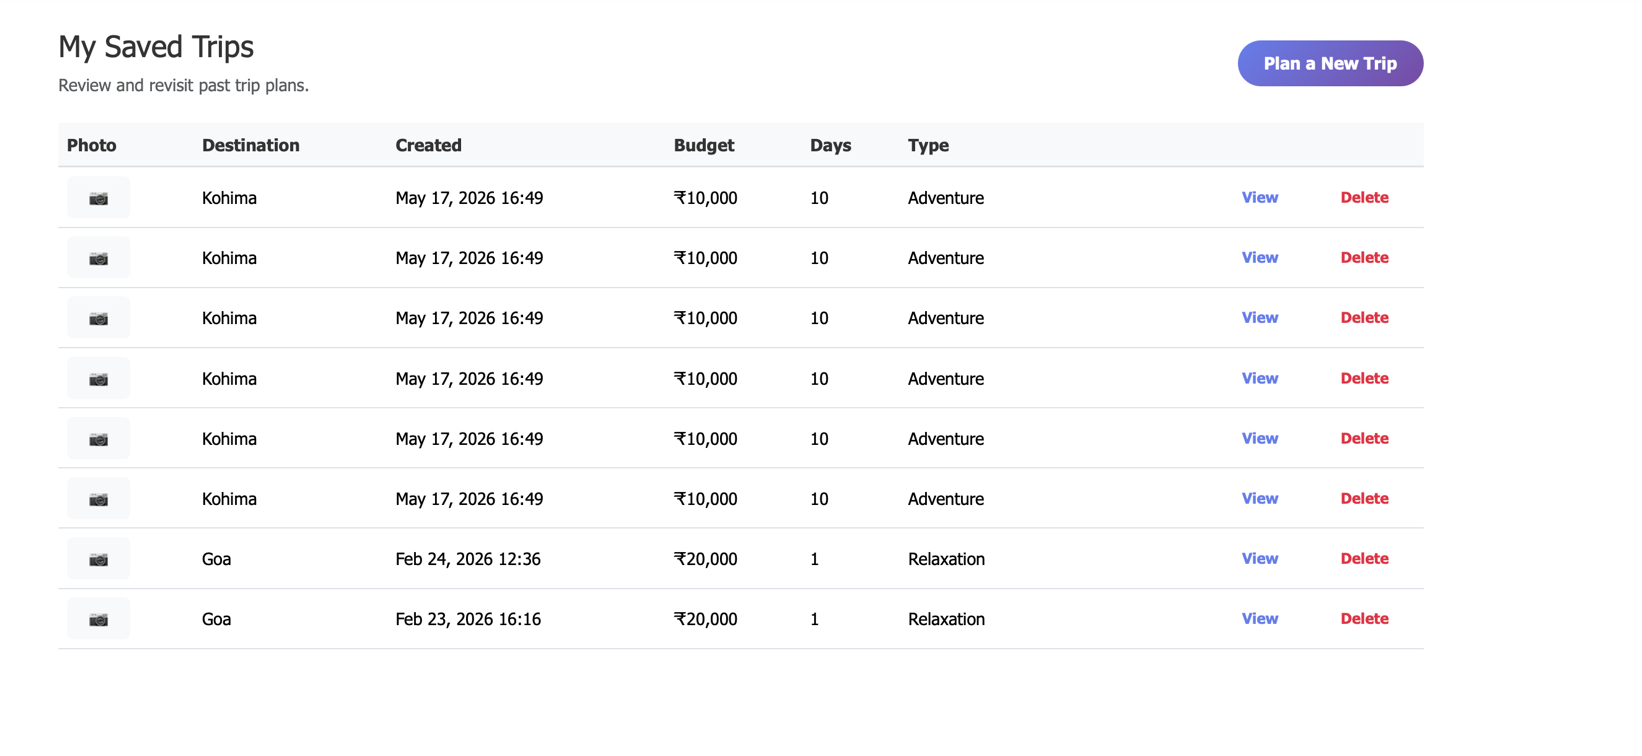
\includegraphics[width=0.9\textwidth,height=0.7\textheight,keepaspectratio]{images/Result View 2.png}
    \caption{Results View - Day-wise Itinerary}
    \label{fig:screenshot-result-2}
\end{figure}

The application visualizes budget distribution using percentages and organized layout structures to improve readability and user understanding. The interface is designed to create an immersive and professional travel planning experience while maintaining performance and responsiveness across all supported devices.
